\begin{frame}
\begin{example}
Let $P_0(a,0,0)$, $P_1(0,b,0)$  $P_2(0,0,c)$ be three points, $a,b,c\neq 0$. Find plane $\mathcal{P}$ passing through $P_0$, $P_1$, $P_2$ (i.e., plane with prescribed $x,y,z$-intercepts).

\bigskip

\begin{columns}
  \column{0.3\textwidth}
        \psfrag{O}{$O$}
        \psfrag{x}{$x$}
        \psfrag{y}{$y$}
        \psfrag{z}{$z$}
        \psfrag{A}{$P_0(a,0,0)$}
        \psfrag{B}{$P_1(0,b,0)$}
        \psfrag{C}{$P_2(0,0,c)$}
        \psfrag{n}{$\textbf{n}$}
        \psfrag{u}{$\textbf{u}$}
        \psfrag{v}{$\textbf{v}$}
        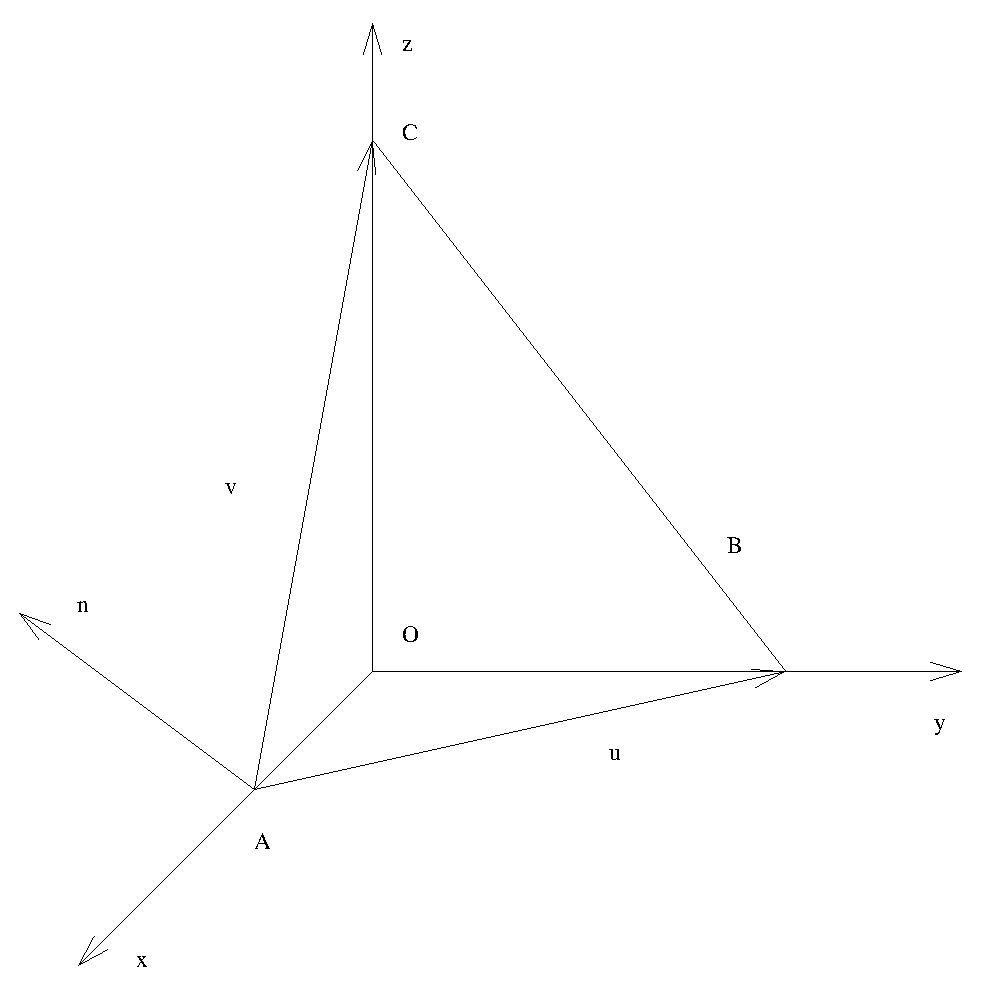
\includegraphics[width=1.5in]{../../modules/vectors/pictures/ok-plane_intercepts.eps}
\column{0.7\textwidth}  
$\mathcal{P}$: parallel to $\textbf{P}_0\textbf{P}_1 = \langle -a, b, 0\rangle, \textbf{P}_0\textbf{P}_2 = \langle -a, 0 c\rangle.$ Normal: 
$$\textbf{n} =\textbf{P}_0\textbf{P}_1 \times \textbf{P}_0\textbf{P}_2=
\left| \begin{array}{ccc}
        \textbf{i} & \textbf{j} & \textbf{k} \\
	-a & b & 0 \\
        -a & 0 & c
       \end{array}
 \right| = bc \textbf{i} + ac \textbf{j} + ab \textbf{k}\; .$$

Implicit scalar equation of plane:
\[
\begin{array}{rcl}
\langle x-a, y, z \rangle \cdot \langle bc, ac, ab \rangle &=& 0\\
bcx+acy + abz &=& abc \\
\frac{x}{a} + \frac{y}{b} + \frac{z}{c} &=& 1
\end{array}
\]
\end{columns}
\end{example}
\end{frame}